\documentclass[12pt]{article}
\usepackage[utf8]{inputenc}
\usepackage[T1]{fontenc}
\usepackage[polish]{babel}
\usepackage{geometry}
\usepackage{tabularx}
\usepackage[table,xcdraw,dvipsnames]{xcolor}
\usepackage{tabularx}
\usepackage{color}
\usepackage{subfig}
\usepackage{sidecap}
\usepackage{wrapfig}
\usepackage{float}
\usepackage{enumerate}
\usepackage{graphicx}
\usepackage{multirow}
\usepackage{hyperref}
\usepackage{titlesec}
\usepackage{amsmath}
\usepackage{anyfontsize}
\usepackage{indentfirst}
\usepackage{listings}
\usepackage{multicol}
\usepackage{pgfplots}
\usepackage{fancyhdr}

\newgeometry{tmargin=1.8cm,bmargin=1.8cm,lmargin =1.8cm,rmargin=1.8cm}
\begin{document}


\begin{table}[H]
    \centering
    \renewcommand{\arraystretch}{1.5}
    \begin{tabularx}{\textwidth}{|X|X|}
    \hline
    \multicolumn{2}{|c|}{\large\textbf{Notatka służbowa nr 1}} \\ \hline
    Temat:          & Sterowniki PLC (TSX Micro 37)     \\ \hline
    Wykonanie:      & Zuzanna Mejer, 259382   \\ \hline
    Termin zajęć:   & poniedziałek TP, 10:55  \\ \hline  
    Data:           & 17.10.2022    \\ \hline
    \end{tabularx}
    \end{table}

\section{Cel ćwiczenia}
Celem ćwiczenia było zaznajomienie się z obsługą sterownika PLC - konfiguracją oraz programowaniem w języku drabinkowym. Podczas ćwiczenia używany był sterownik TSX Micro 3721 firmy Schneider Automation z oprogramowaniem w wersji V1.6. Do zapoznawania się z podstawami języka drabinkowego korzystano z programu PL7PRO. 

\section{Uruchomienie oprogramowania i konfiguracja sterownika}
Przed rozpoczęciem pracy ze sterownikiem, należało uruchomić i skonfigurować oprogramowanie i sterownik. W tym celu wykonano poniższe czynności.

\begin{enumerate}
    \item Uruchomiono program PL7PRO i utworzono nowy projekt. Pojawiło się okno, w którym należało wybrać odpowiedni sterownik (TSX Micro), model wraz z wersją oprogramowania (TSX 3721 V1.5 - ze względu na brak wersji V1.6) oraz zaznaczyć ,,No'' przy Grafcet. Przedstawia to poniższe zdjęcie.
    \begin{figure}[H]
        \centering
        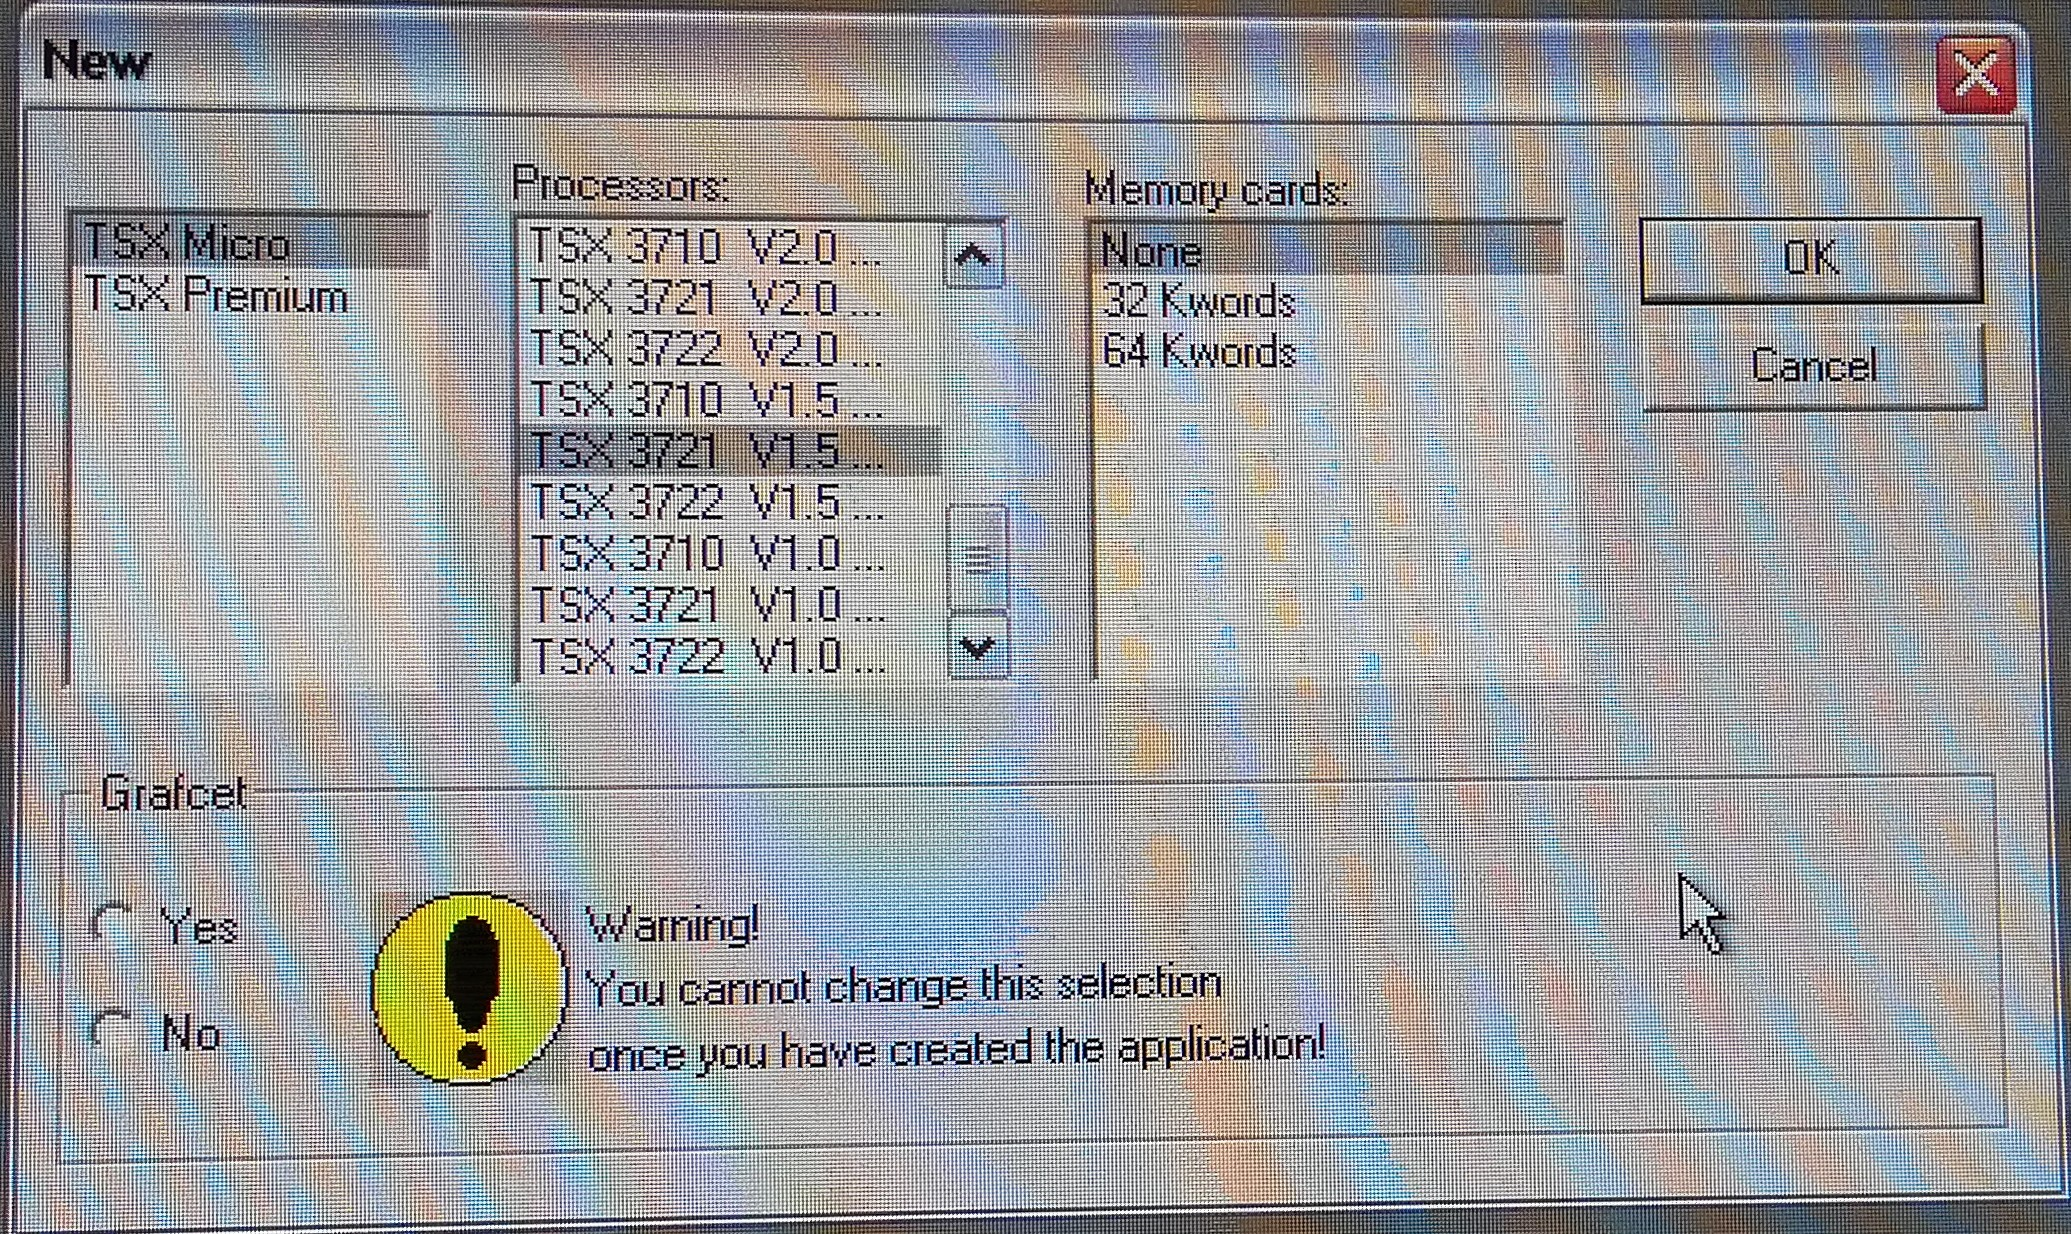
\includegraphics[scale=0.20]{konfiguracja.jpg}
        \caption{Uruchomienie programu}
    \end{figure}


    \item Następnie zdefiniowano typy modułów sterownika. Wybrano opcję \textit{Configuration $ \rightarrow $ Hardware configuration} i wpisano odpowiednie typy modułów. W przypadku stanowiska pierwszego były one następujące: 
    \begin{itemize}
        \item moduł wejść i wyjść cyfrowych - TSX DMZ 28DR
        \item moduł wejść analogowych - TSX AEZ 414
        \item moduł wyjść analogowych - TSX ASZ 200
    \end{itemize}
    \item Wybrano język programowania drabinkowy i przećwiczono podstawy obsługi programu oraz przesyłanie programu do sterownika i uruchamianie go.
\end{enumerate}

\section{Podstawowe funkcje logiczne i układy czasowe}
Po zakończonej konfiguracji programu i sterownika, na fragmencie linii produkcyjnej wykonywano zadania dostępne w instrukcji laboratoryjnej.

\subsection{Zadanie wprowadzające}
Dane były trzy układy do przetestowania i przeanalizowania:

\begin{figure}[H]
    \centering
    \subfloat[]{
        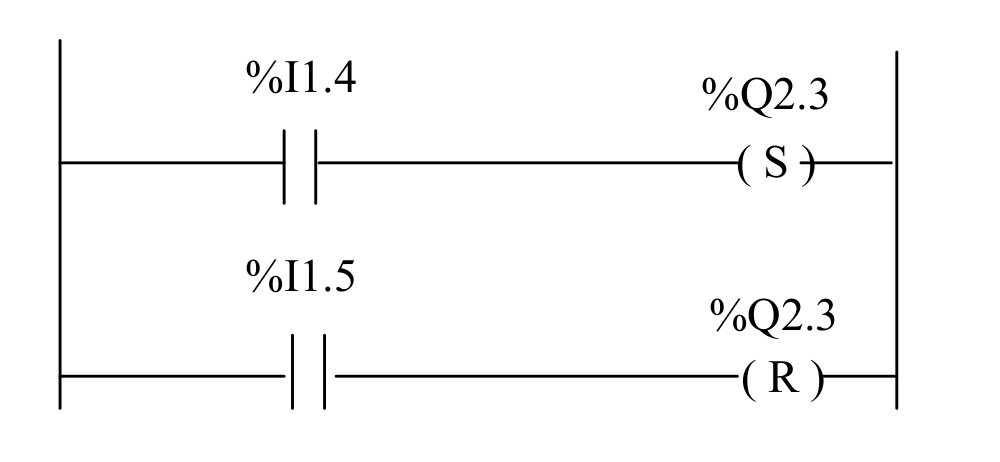
\includegraphics[scale=0.25]{2a.png}
        \label{a}}
    \subfloat[]{
        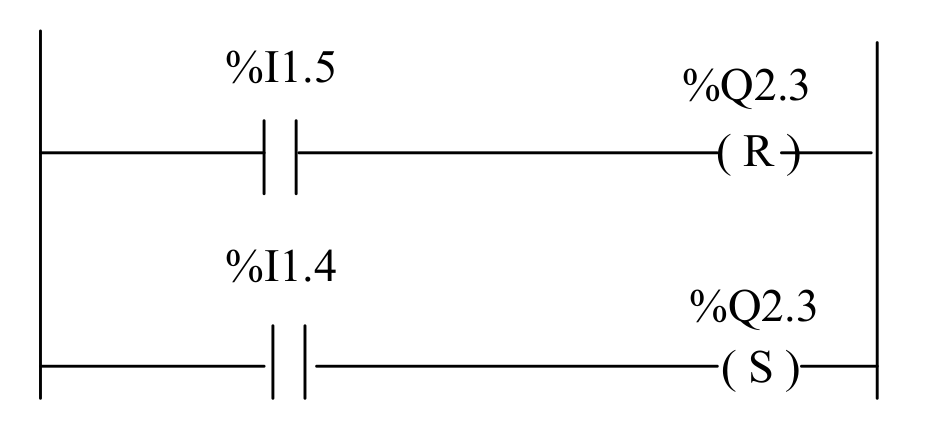
\includegraphics[scale=0.25]{2b.png}
        \label{b}}
    \quad
    \subfloat[]{
        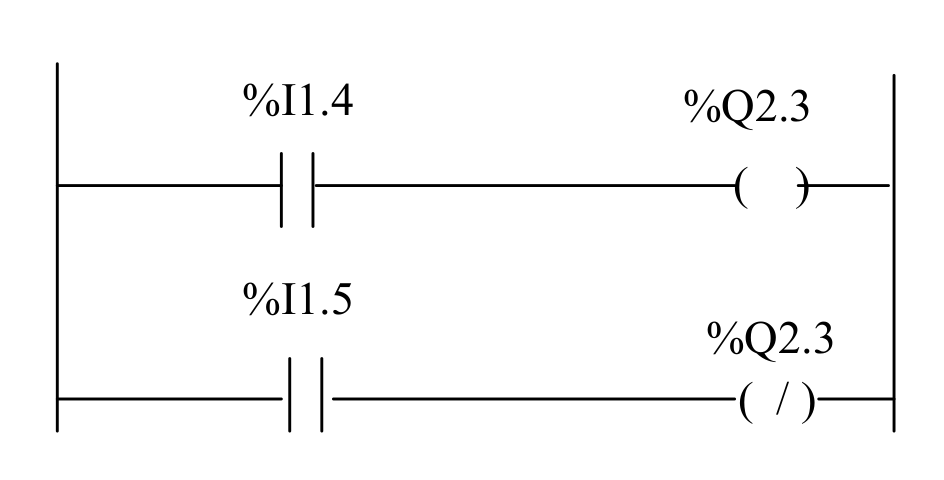
\includegraphics[scale=0.25]{2c.png}
        \label{c}}
    \caption{Układy do przeanalizowania}
\end{figure}

W programowaniu w języku drabinkowym należy pamiętać o tym, że sterownik wykonuje działania kolejno od górnego szczebla w kierunku dolnego. Różnica pomiędzy układami \ref{a} a \ref{b} polega na zamienieniu kolejności szczebli. Układ \ref{b} nie zadziała poprawnie, ze względu na to, że program najpierw zrobi reset cewki $\%Q2.3$, a dopiero potem set.

W układzie \ref{c} wciśnięcie przycisku $\%I1.4$ zaktywuje zmienną $\%Q2.3$ do momentu, aż przycisk nie zostanie puszczony. Wciśnięcie przycisku $\%I1.5$ zaneguje zmienną $\%Q2.3$. W praktyce na fragmencie linii produkcyjnej należało przycisnąć guziki wystarczająco długo, aby wykonał się pełen ruch.

\subsection{Timery}
W języku Ladder są dostępne trzy układy czasowe: TON, TOF oraz TP. Ich działanie zostało przetestowane oraz opisane poniżej.

\subsubsection{Timer On-Delay (TON) - opóźnione zadziałanie}

Układ TON został przedstawiony poniżej:

\begin{figure}[H]
    \centering
    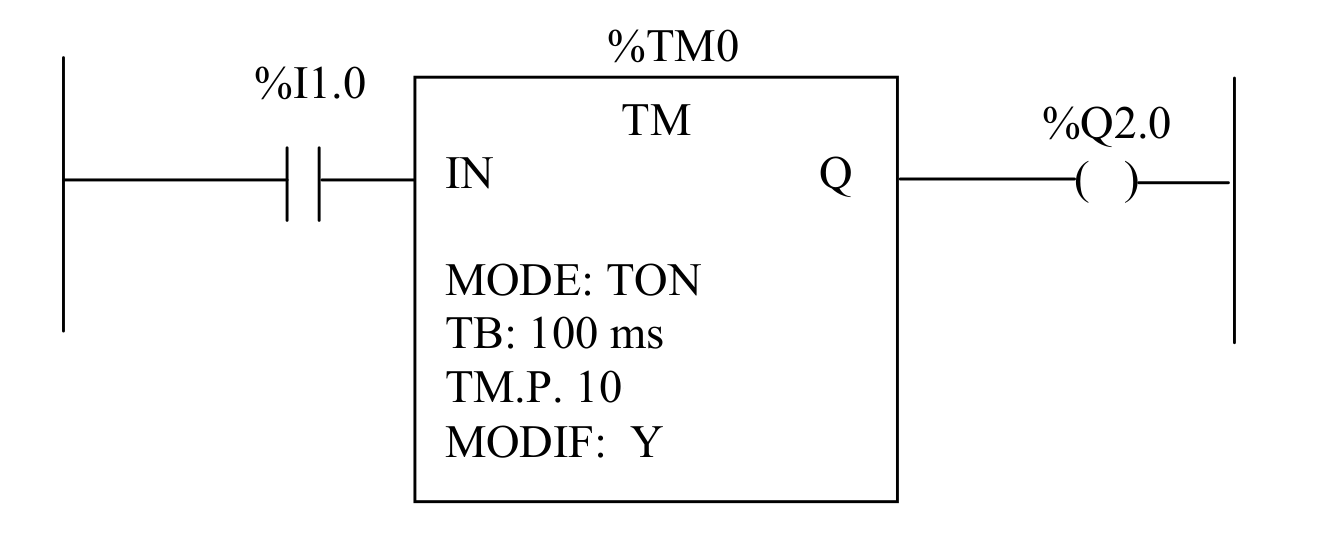
\includegraphics[scale=0.25]{ton.png}
    \caption{Timer On-Delay}
\end{figure}

Parametr \textit{TB} to czas bazowy, ustawiony tutaj na 100 ms. \textit{TM.P} to wartość zadana. Na podstawie tych parametrów obliczany jest czas opóźnienia:
$ TB \cdot TM.P = 100 ms \cdot 10 = 1000 ms = 1s $. W tym przypadku opóźnienie ustawiono na 1s. Timer On-Delay opóźnia działanie o podany czas. To oznacza, że po wciśnięciu przycisku $\%I1.0$, timer odmierzył 1 sekundę i dopiero po tym czasie zaktywował zmienną $\%Q2.0$.


\subsubsection{Timer Off-Delay (TOF) - opóźnione wyłączenie}

Układ TOF został przedstawiony poniżej:

\begin{figure}[H]
    \centering
    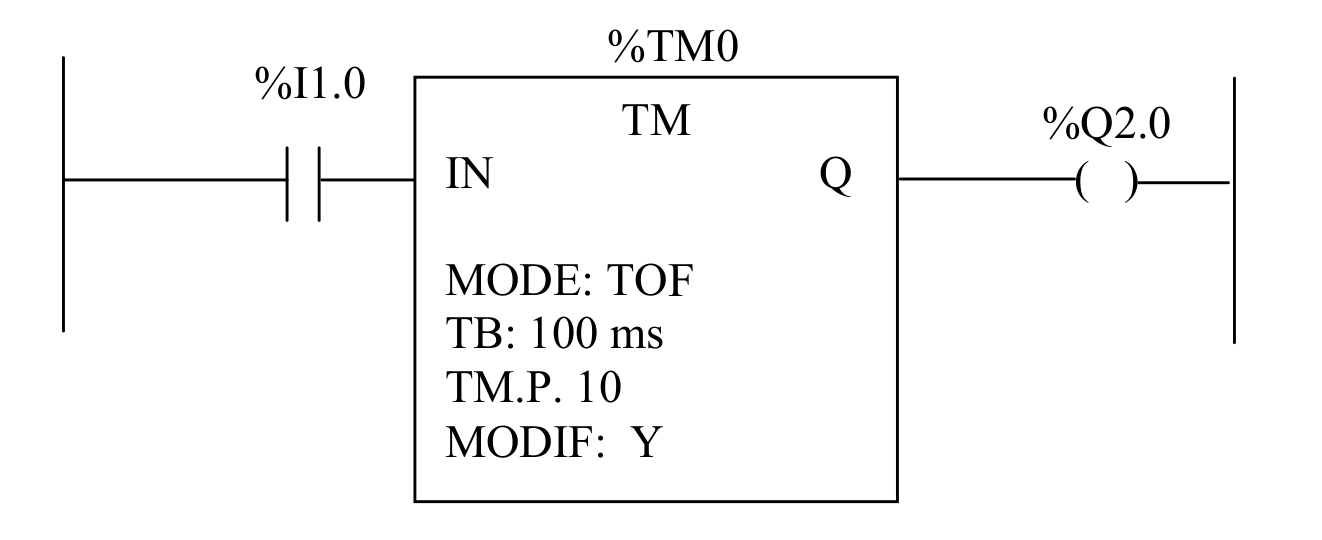
\includegraphics[scale=0.25]{tof.png}
    \caption{Timer Off-Delay}
\end{figure}

Po wciśnięciu przycisku $\%I1.0$ program od razu aktywuje zmienną $\%Q2.0$ i wyłącza program po odliczeniu czasu wyliczonego jako $ TB \cdot TM.P $. 

\colorbox{WildStrawberry}{przebiegi?}

\subsubsection{Timer Pulse (TP) - puls}

Układ TP został przedstawiony poniżej:

\begin{figure}[H]
    \centering
    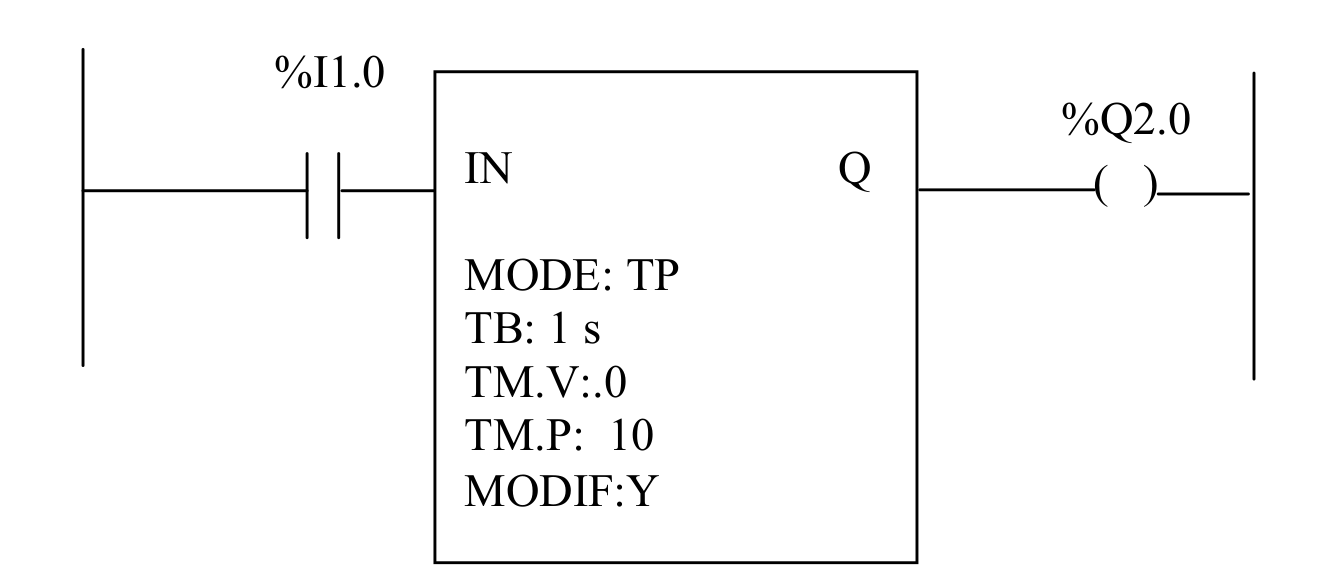
\includegraphics[scale=0.25]{tp.png}
    \caption{Timer Pulse}
\end{figure}

Parametr \textit{TMi.V} to bieżąca wartość timera. Timer ten działa pulsacyjnie, to znaczy, że każda operacja trwa określoną długość (w tym przypadku 10s) i następnie przełącza się na wykonywanie kolejnej operacji. 

\subsection{Przykład zmiany stałej PRESET Timera przy pomocy funkcji \textit{operate}}

Zbudowany został następujący układ:

\begin{figure}[H]
    \centering
    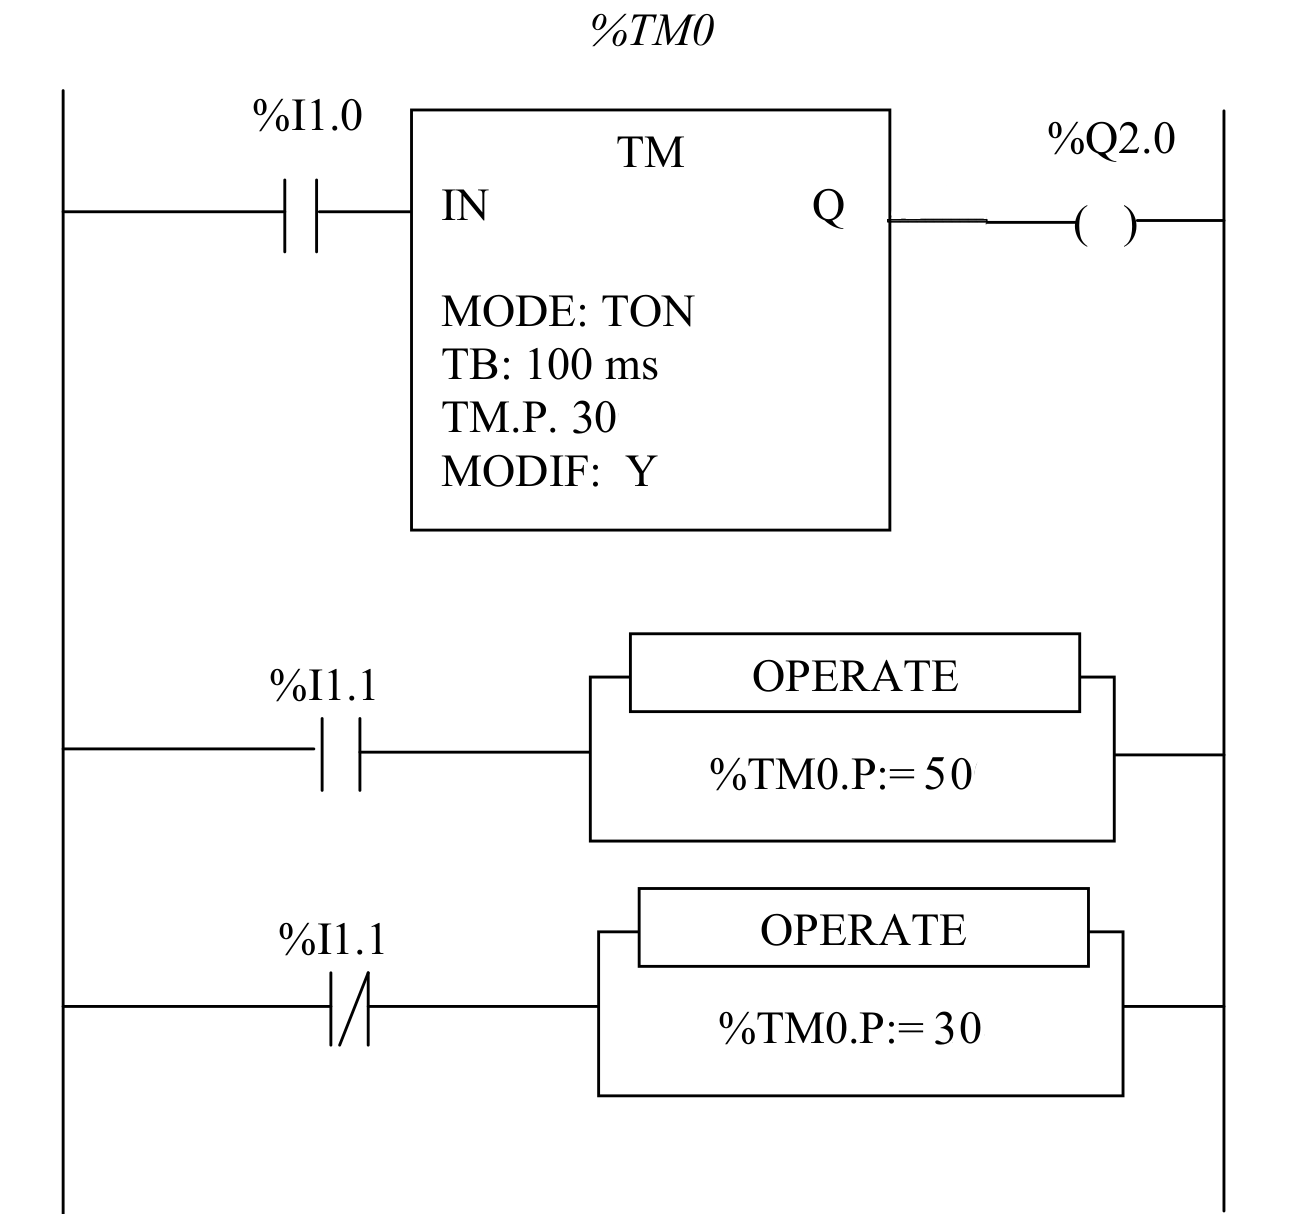
\includegraphics[scale=0.25]{operate.png}
    \caption{Zmiana stałej PRESET Timera przy pomocy funkcji \textit{operate}}
\end{figure}

Poniżej przedstawiono zdjęcie programu:

\begin{figure}[H]
    \centering
    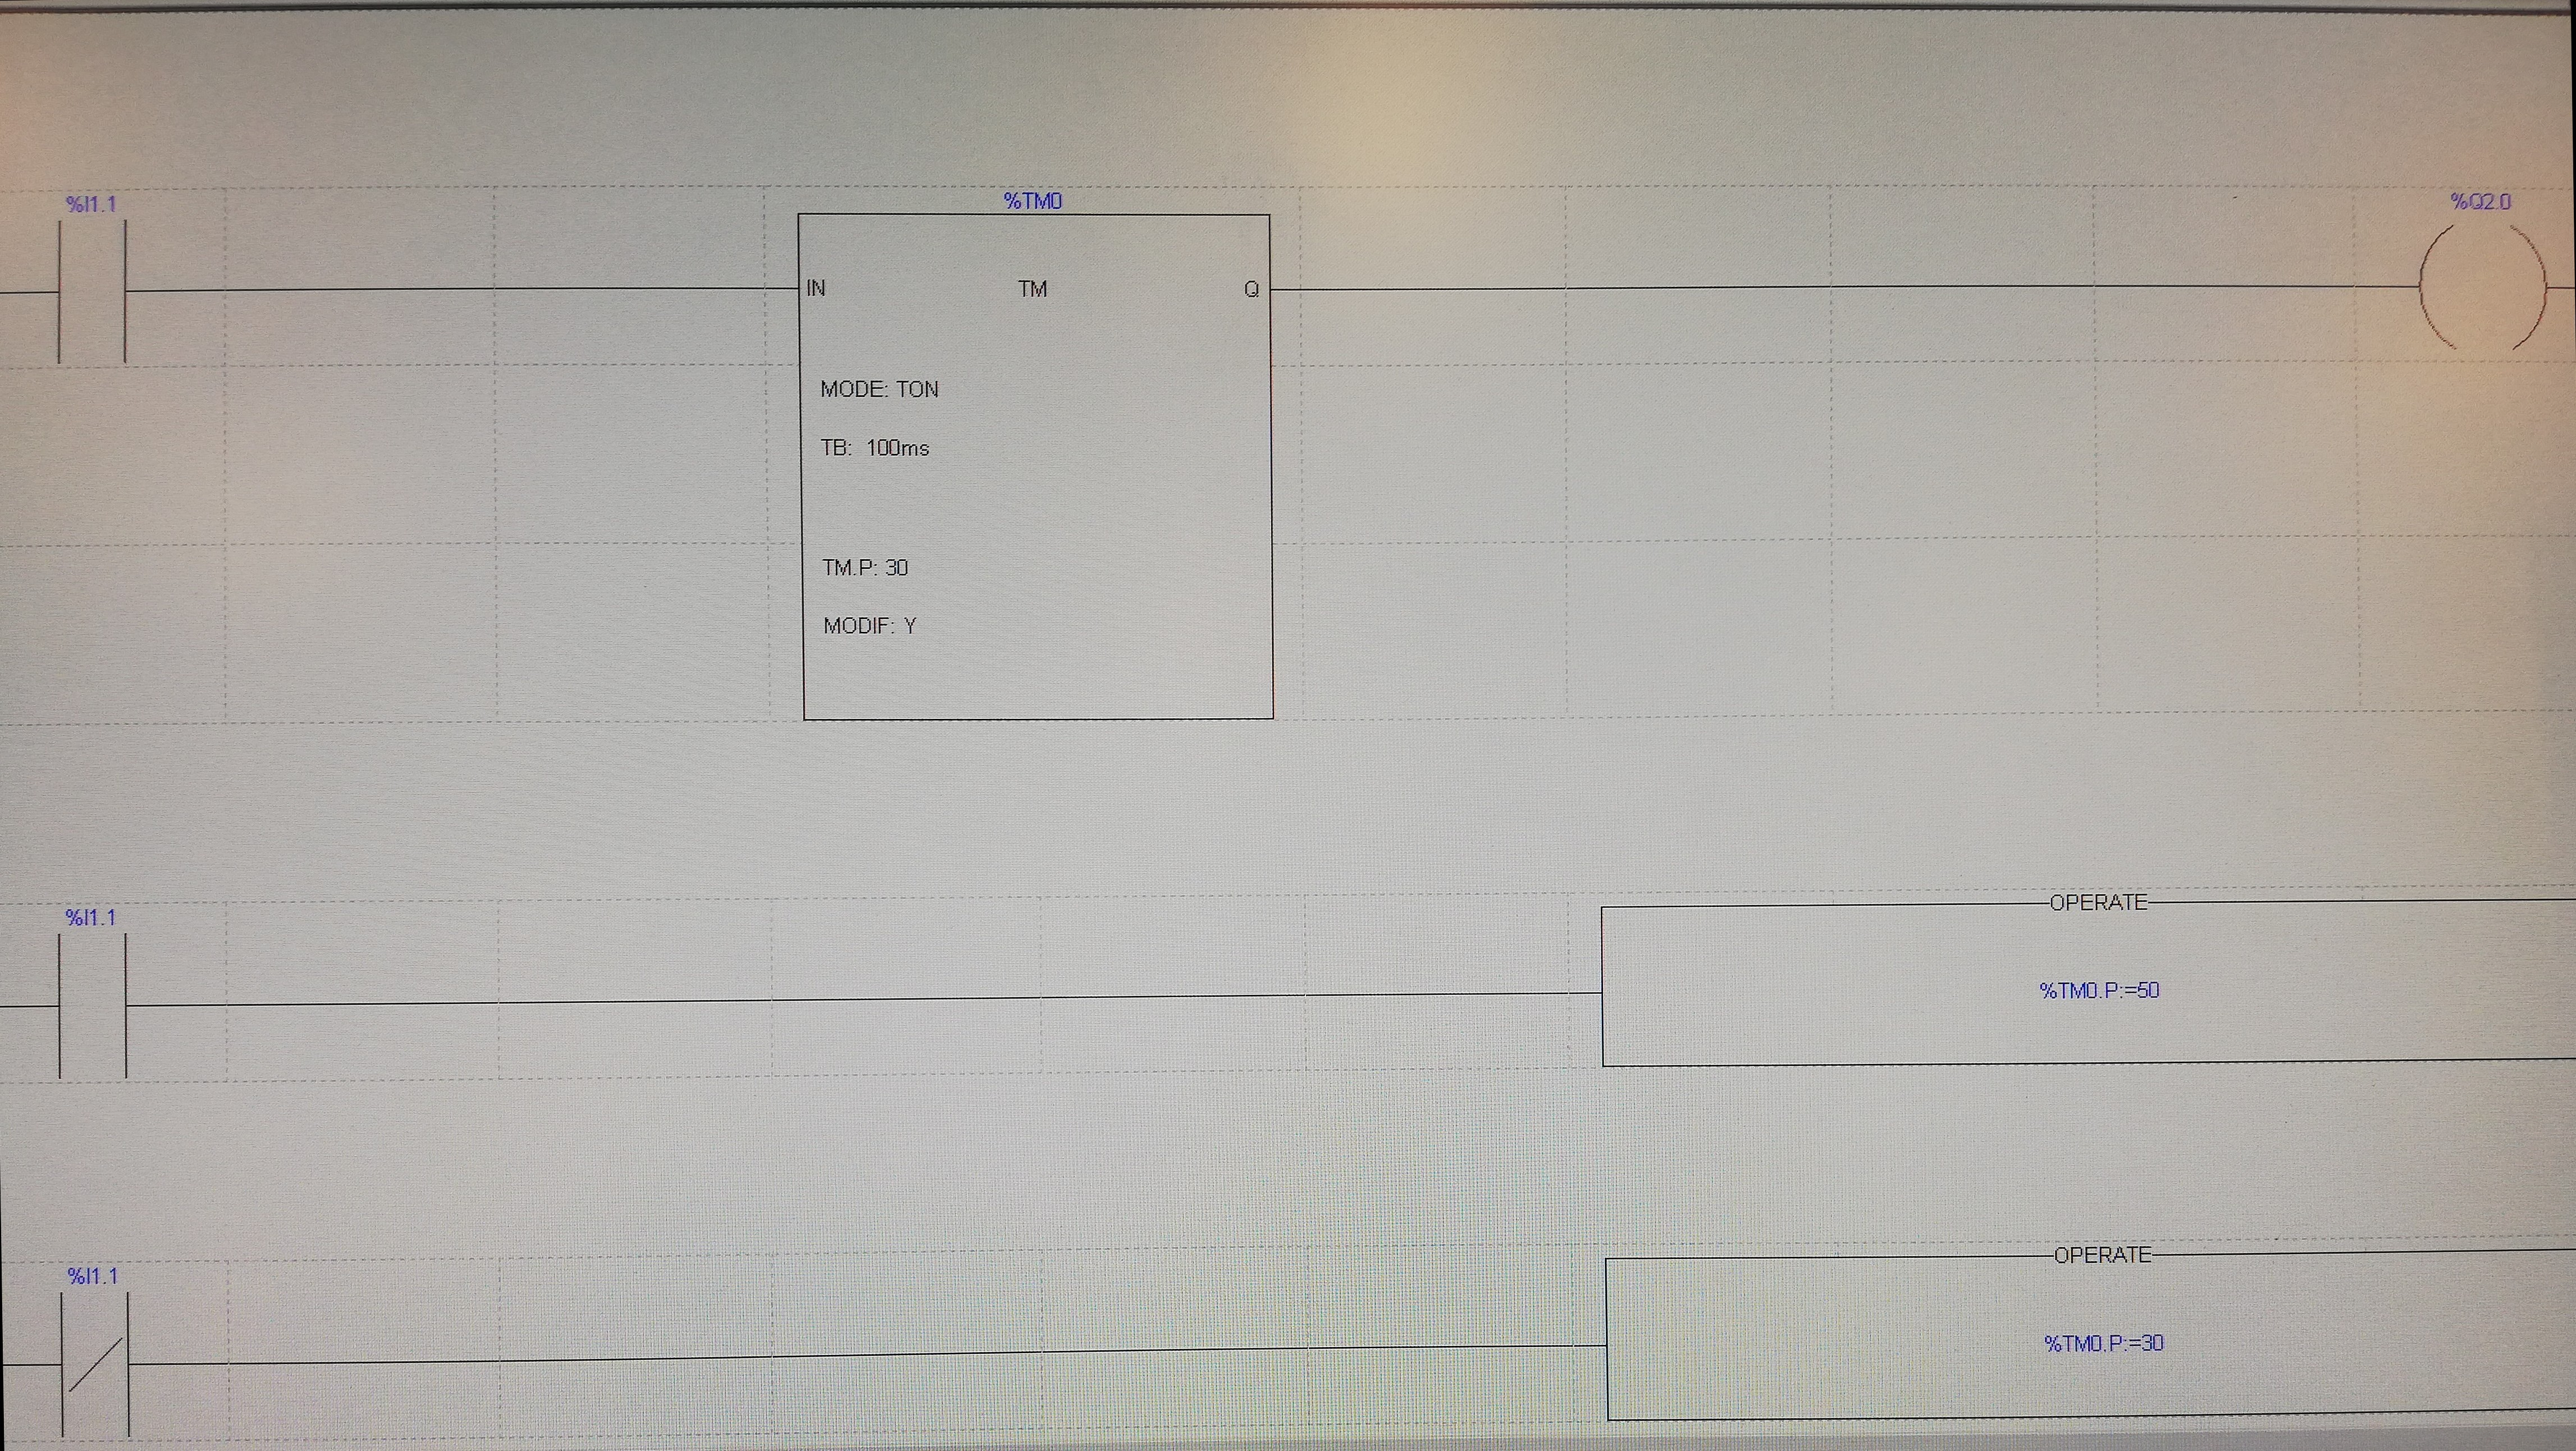
\includegraphics[width=\textwidth]{operate_zdj.jpg}
    \caption{Realizacja zmiany stałej Timera przy pomocy funkcji \textit{operate}}
\end{figure}

Funkcja \textit{operate} służy do zamiany wartości zadanej TM.P po przyciśnięciu $\%I1.1$ na wartość 50 i po puszczeniu - z powrotem na wartość 30. Jeśli wciśnięty jest $\%I1.1$ i $\%I1.0$, licznik odlicza 5 sekund, po czym aktywuje $\%Q2$. Jeśli natomiast wciśnięty jest jedynie $\%I1.0$, licznik odmierza 3 sekundy.


\subsection{Liczniki}

Opracowano następujący układ licznika:
\begin{figure}[H]
    \centering
    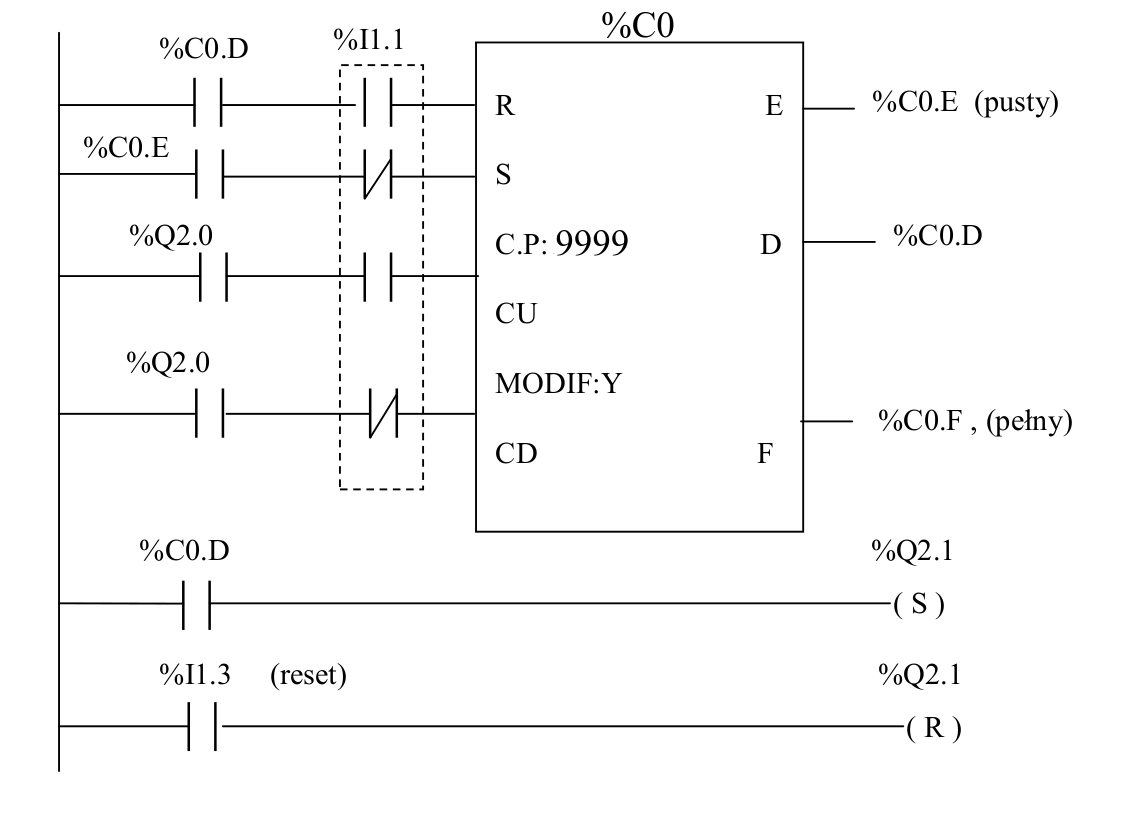
\includegraphics[scale=0.35]{licznik.png}
    \caption{}
\end{figure}

Poniżej przedstawiono jego realizację w programie:
\begin{figure}[H]
    \centering
    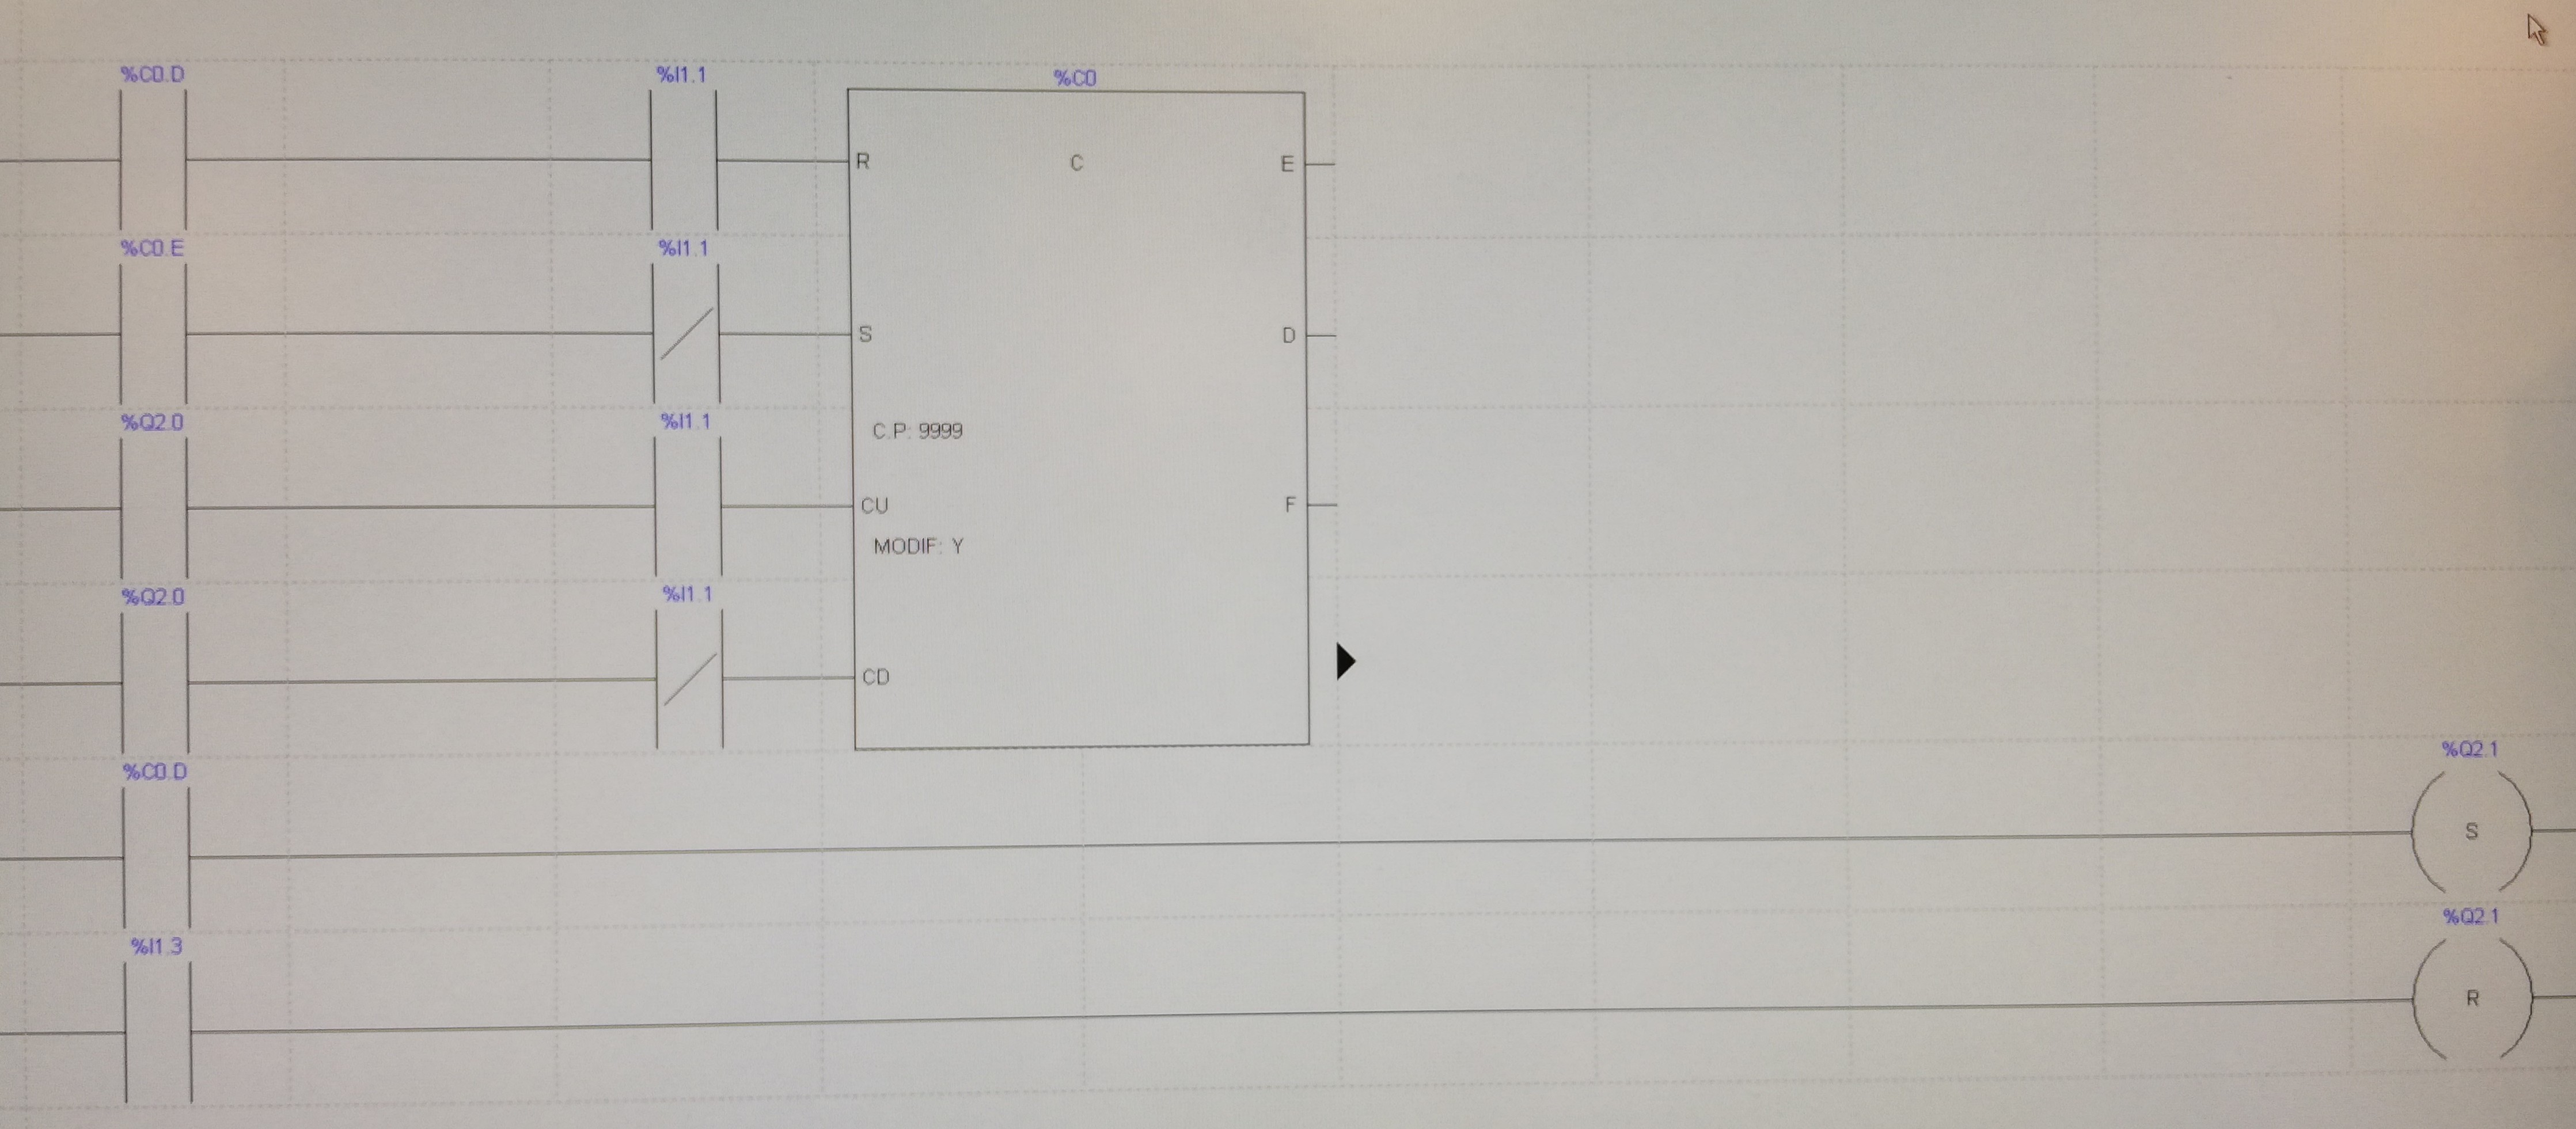
\includegraphics[width=\textwidth]{licznik_zdj.jpg}
    \caption{Realizacja licznika w programie}
\end{figure}

Ponadto, zbudowano generator do testowania licznika zdarzeń, co przedstawia poniższe zdjęcie:
\begin{figure}[H]
    \centering
    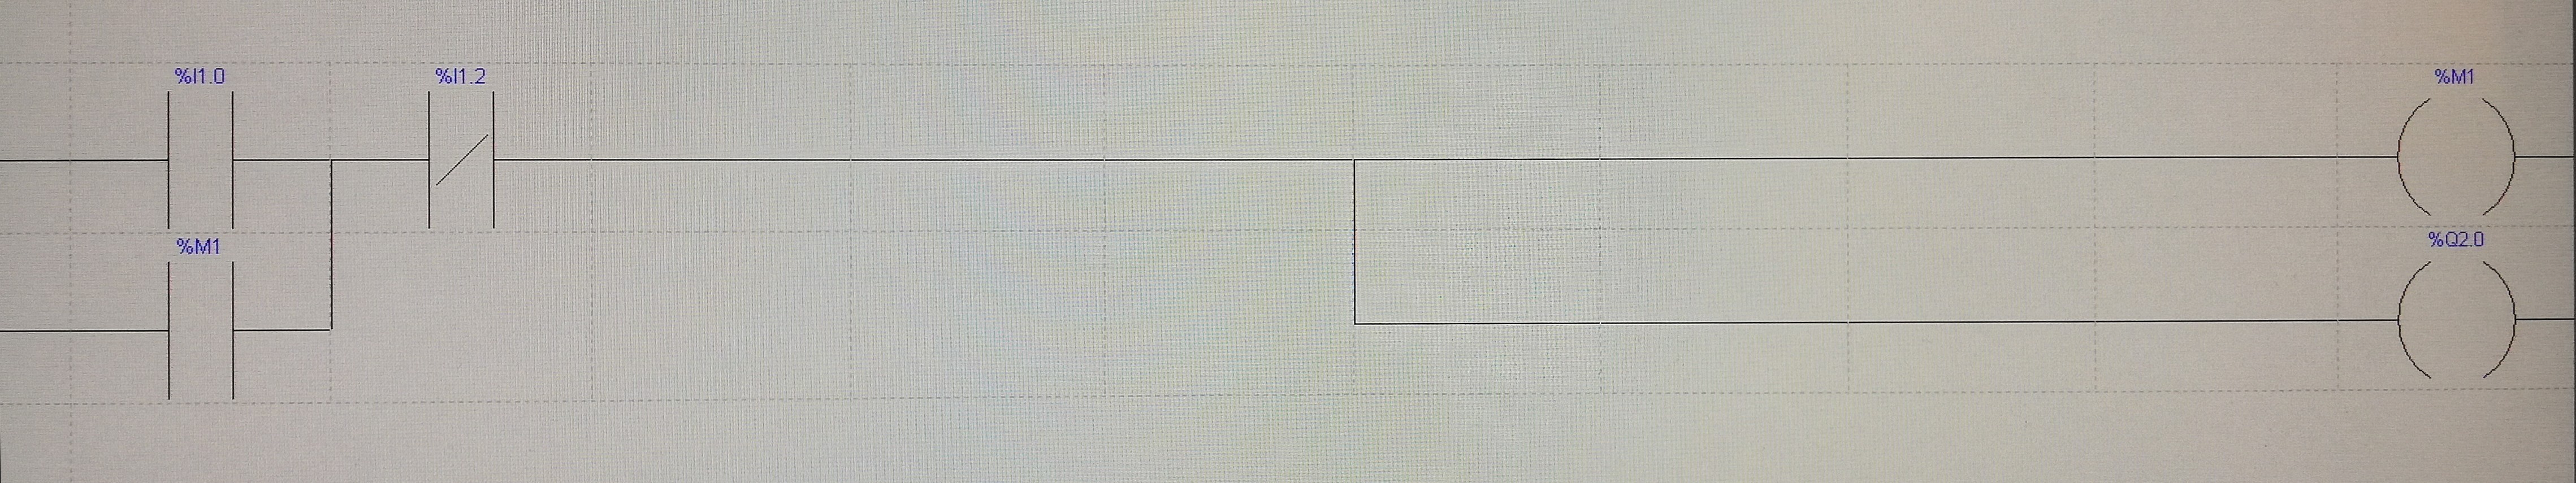
\includegraphics[width=\textwidth]{licznik_zdj2.jpg}
    \caption{Realizacja generatora do testowania licznika zdarzeń}
\end{figure}

Podczas zajęć zabrakło czasu, żeby przetestować działanie licznika i napisanego fragmentu programu.


\section{Podsumowanie}
Zajęcia poświęcone były wprowadzeniu do obsługi sterowników PLC oraz do języka drabinkowego. Podczas zajęć zaznajomiono się z podstawowymi funkcjami logicznymi, układami czasowymi oraz licznikami. Zadania nie sprawiły problemów.



\end{document}